\documentclass[OPS,toc,lsstdraft,authoryear]{lsstdoc}
% lsstdoc documentation: https://lsst-texmf.lsst.io/lsstdoc.html

% Generated by Makefile
\input{meta}

% Package imports go here.
\usepackage{graphicx}
\usepackage{float}

% Local commands go here.
\graphicspath{{figures/}} %Setting the graphicspath

% If you want glossaries, uncomment:
% \input{aglossary.tex}
% \makeglossaries

\title{Rubin Observatory Risk and Opportunity Management Plan}
% \setDocSubtitle{Optional subtitle}

\author{%
Austin Roberts,
Robert Blum,
Chuck Claver,
Leanne Guy,
Phil Marshall,
Wil O'Mullane,
Kevin Siruno,
Matthew Rumore.
}

\setDocRef{RDO-71}
\setDocUpstreamLocation{\url{https://github.com/lsst/RDO-71}}
\date{\vcsDate}
\setDocCurator{TBD}

\setDocAbstract{%
The document provides the Rubin Observatory Risk and Opportunity Management Plan.
}

% Revision history.
% Order: oldest first.
% Fields: VERSION, DATE, DESCRIPTION, OWNER NAME.
% See LPM-51 for version number policy.
\setDocChangeRecord{%
  \addtohist{1.0}{2022-12-12}{Unreleased draft.}{Matthew Rumore}
  \addtohist{2.0}{2024-03-26}{First release preparation.}{Matthew Rumore}
  \addtohist{2.1}{2024-04-03}{Impact analysis and budgeting.}{Phil Marshall}
  \addtohist{2.2}{2024-04-05}{Finalize main content for first release.}{Matthew Rumore, Leanne Guy}
}

\begin{document}

\maketitle



\section{Introduction and Background}

This document describes the Risk \& Opportunity Management Plan used to identify, assess, respond to, and manage risks and opportunities associated with the technical, cost and schedule aspects for the Vera C.\ Rubin Observatory throughout the operation of the Legacy Survey of Space and Time (LSST).
The Rubin Observatory Risk \& Opportunity Management Plan recognizes the benefits of managing uncertainty during operations in a holistic and systematic manner.

The Risk \& Opportunity Management Plan is one plan in a group of Rubin Observatory Operations plans that collectively define a comprehensive approach to managing risk, and opportunity, which are collectively known as approaches to making decisions under conditions of uncertainty.
Risk of harm to personnel and equipment is the focus of the Rubin Observatory Safety Policy, \citeds{RDO-015}.
Further aspects of risk and safety management are codified under the NSF (National Science Foundation) NOIRLab and the Department of Energy (DOE) SLAC Laboratory (SLAC National Accelerator Laboratory) documents where appropriate. 
Additionally and were applicable,  risk, safety, and hazard analysis plans are adopted for Rubin Observatory Operations from the Rubin Observatory Construction Project .

The key aspects of the Risk \& Opportunity Management Plan are:
\begin{itemize}
	\item A standard methodology to identify and assess major risks and opportunities associated with Operations work breakdown structure (WBS) elements and operations functions from the Operations Plan.

	\item A continuous process to review and re-assess current risks and opportunities on a quarterly or semi-annual basis and address new risks and opportunities as they emerge.
	
	\item Common techniques for assignment of budget and schedule for the anticipated response in the event of a realized risk.
	
	\item An approach and tool to measure and compare to contingency levels, the remaining major risk exposure across operation.
	
	\item A single dynamic and interactive system to inform management, to support communication across operations, to facilitate and encourage regular participation of team members, and to produce standard reporting and tracking features.
\end{itemize}


\subsection{Risk Management Process Overview}

The risk management process is a continuous and proactive approach to keeping risk at an acceptable level through awareness, tracking, and response handling.
The Rubin Observatory Risk Management process is an event-centric approach.
It is characterized by the identification of events that may occur in the future with resulting negative or positive consequences for operations.
There are different types of risk associated with Rubin Observatory Operations:
\begin{itemize}
\item Technical Risk, consisting of the risk of not meeting survey performance requirements or deliverables;
\item Cost Risk, consisting of the risk that the available budget will be insufficient to cover the scope of operations;
\item Schedule Risk, consisting of the risk that the survey will fail to meet scheduled milestones; and,
\item a related category of risk is called Programmatic Risk, which is risk produced by events that are beyond the control of the operations management team, where programmatic Risk can be a source of risk in any of the other three risk categories. 
\end{itemize}

In transitioning from the construction phase to operations, the operations team will consult with the Rubin Observatory  project to understand any project risks that might transfer to operations or (more likely) evolve into operations risks.
During the pre-operations phase, which occurs in parallel with the project integration and commissioning phases, the operations team will work closely with the project team to understand all risks, safety plans, and hazards and adapt, revise, and establish analogous processes, procedures, and policies.
This transition will take place from the beginning of pre-operations and be completed no later than the Operations Readiness Review (ORR), which marks formal handover of the Rubin Observatory system from the project to the operations team.

\subsection{Risk Management Tools}

Rubin Observatory Operations will follow the NOIRLab model, shown Figure \ref{fig:NOIRLab-risk-model} for managing its risks and opportunities. 
The Alcea Tracking Solutions (ATS) software tool for risk management, which has been adopted by NOIRLab, will used by Rubin.   
The user guide for the ATS  tool is found in \citeds{RTN-051}.

In addition to this, Rubin may choose to implement additional tools on top of the Alcea tool to better integrate the process of risk and opportunity management into the Rubin workflow. 
Any additional such tools developed by Rubin for managing risks will be added to this document as they are developed. 
 
All risks are reported to AURA and SLAC management, as well as NSF through NOIRLab quarterly reports.

\begin{figure}[t]
\caption{NOIRLab Risk Management Model.}
\centering
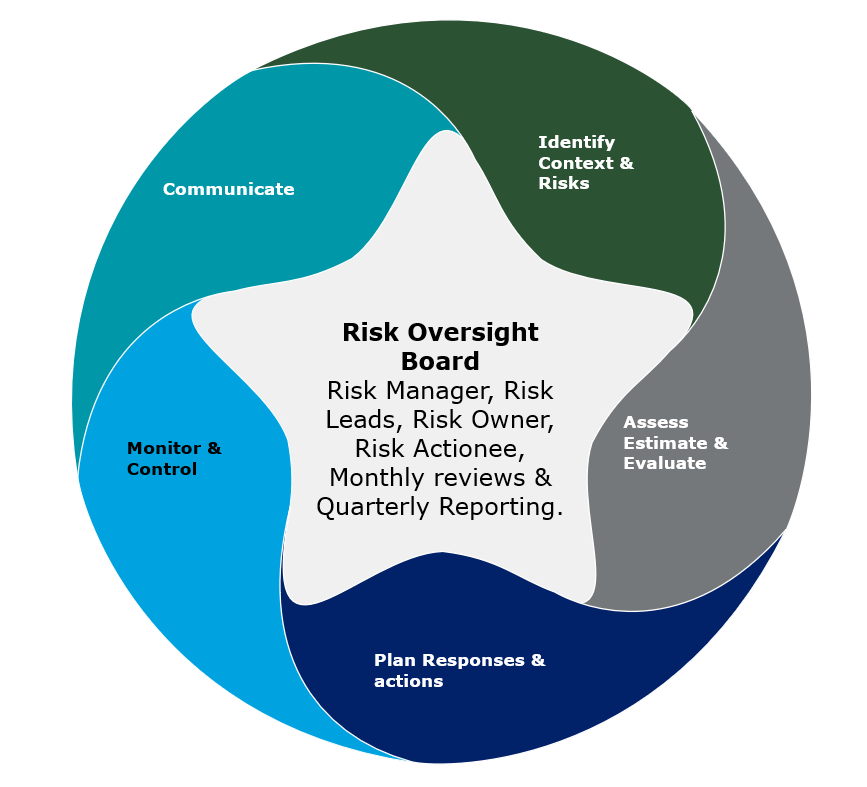
\includegraphics[width=\textwidth]{NOIRLab-risk-model-temp}
\label{fig:NOIRLab-risk-model}
\end{figure}


\subsection{Roles and Responsibilities}

The Rubin Observatory Risk \& Opportunity Board (RROB) serves as the managing group for the Risk \& Opportunity Management Plan.
The RROB is managed by the System Performance (SP) Department.

The \textbf{Rubin Observatory Operations Director} has overall responsibility for managing and controlling operations risks.
The Director will work with the senior managers to review and assess current risks on a quarterly basis.
The Director will also approve all new risks (or delegate this responsibility as appropriate to another operations manager) in coordination with the RROB.

The \textbf{Rubin Observatory Executive Council} is the group of operations management and leadership staff charged with reviewing the risk registry, evaluating the risk and opportunity assessments, collaborating on risk handling options, and developing implementation recommendations, which are forwarded to the Director of operations.
The Executive Council consists of the Associate Directors (ADs) and Deputy Directors as well as other operations staff.
It is expected that the head of safety for NOIRLab will meet with the Executive Council to regularly review risks.



\subsection{Risk \& Opportunity Definitions}
\label{sec:definitions}

\textbf{Risk} (also known as \textbf{Threat}) ---
The degree of exposure to an event that might happen to the \emph{detriment} of a program, project, or other activity. 
It is described by a combination of the probability that the risk event will occur and the consequence of the extent of loss from the occurrence, or impact.
Risk is an inherent part of all activities, whether the activity is simple and small, or large and complex.
Risks are categorized into four types depending on how they impact operations --- technical, budget (cost), schedule and programmatic.

The term \emph{risk} is used in this document to refer to a risk that has a negative impact, also known as a "threat". 
The term "risk" that has a positive impact is an \emph{opportunity}, and is described below.

\textbf{Issue} ---
A risk that has been realized, e.g. the undesired outcome has materialized.

\textbf{Technical Risk} ---
The possibility that a technical requirement of the system may not be achieved in the system life cycle.
Technical risk exists if the system may fail to achieve performance requirements; to meet operability, producibility, testability, or integration requirements; or to meet environmental protection requirements.
A potential failure to meet any requirement that can be expressed in technical terms is a source of technical risk (INCOSE, pg. 220).

\textbf{Budget (Cost) Risk} ---
The possibility that available budget for operations will be reduced or insufficient to cover operations activity.
Cost risk exists if: a) Rubin Observatory must devote more resources than planned to achieve technical requirements; b) Rubin Observatory must add resources to support slipped schedules due to any reason; c) if changes must be made to the scope of operations; or d) if changes occur in the organization (i.e., Rubin Observatory, Association of Universities for Research in Astronomy [AURA] and/or NOIRLab, SLAC) or national economy.
Budget risk can be predicted at the total operations level or for a system element or activity.
The collective effects of activity or element-level cost risk can produce cost risk for Rubin Observatory generally (INCOSE, pg. 220).

\textbf{Schedule Risk} ---
The possibility that Rubin Observatory will fail to meet scheduled milestones.
Schedule risk exists if there is inadequate allowance for delays in survey execution.
Schedule risk exists if difficulty is experienced in achieving schedule accomplishments, such as the timely accumulation of survey data or data release.
Schedule risk can be incurred at the total operations level for milestones such as deployment of the first data release.
The cascading effects of activity or element-level schedule risks can produce schedule risk for Rubin Observatory generally (INCOSE, pg. 220).

\textbf{Programmatic Risk} ---
Produced by events that are beyond the control of the Rubin Observatory management team.
These events often are produced by decisions made by personnel at higher levels of authority, such as reductions in Rubin Observatory priority, delays in receiving authorization to proceed with a change to the operations plan, reduced or delayed funding, changes in organization or national objectives, etc.
Programmatic risk can be a source of risk in any of the other three risk categories (INCOSE, pg. 220).
AURA holds an independent risk register for Rubin Observatory Operations.

\textbf{Risk Management} ---
The art and science of planning, assessing, and handling future events to avoid unfavorable impacts on Rubin Observatory budget, schedule, or performance to the extent possible.
Risk management is a structured, formal, and disciplined activity focused on the necessary steps and planning actions to determine and control risks to an acceptable level.
Risk Management is an event-based management approach to managing uncertainty.

\textbf{Risk and Opportunity Responses} ---
Responses are strategic process(es) controlling identified risks, whereby the stakeholders decide how to deal with each risk be it opportunities or threats.

\textbf{Risk and Opportunity Actions} ---
Actions taken to implement a response plan if a threat or opportunity is realized.

Described below are the four basic response types to risks (threats).

\textbf{Avoidance} ---
Avoid the risk through the change of requirements or redesign (INCOSE, pg. 223).

\textbf{Mitigation} (also known as \textbf{Control}) ---
Requires the expenditure of budget or other resources to reduce the likelihood and/or consequence.
Mitigations are proposed activities that are not part of the operations baseline.
Once mitigation activities are approved, they are just baselined activities and no longer referred to as mitigations.

\textbf{Transfer} ---
Transferring responsibility for the risk by agreement with another party that it is in their scope to mitigate and respond to impacts if the risk is realized. Purchasing insurance is an example of transferring risk.

\textbf{Acceptance} ---
Accept the risk and the consequences of it becoming realized.

% \textbf{Existential Risk} ---

\textbf{Opportunity} (also known as \textbf{Benefit} ---
The degree of exposure to an event that might happen to the benefit of a program, project, or other activity.
It is described by a combination of the probability that the opportunity event will occur and the consequence of the extent of gain from the occurrence, or impact.
There are two levels of opportunities. At the macro level, a project itself is the manifestation of the pursuit of an opportunity.
At the element level, tactical opportunities exist, whereby certain events, if realized, provide a cost or schedule savings to the project or increase survey performance.

\textbf{Opportunity Management} ---
The proactive art and science of planning, assessing, and handling future events to seek favorable impacts on project, cost, schedule, or performance to the extent possible.
Opportunity management is a structured, formal, and disciplined activity focused on the necessary steps and planning actions to determine and exploit opportunities to the extent possible.

Described below are the four basic response types to opportunities.

\textbf{Exploit} ---
Increase the likelihood of the opportunity occurring through the expenditure of budget or other resources.
The expenditure of budget should be evaluated against the probability weighted exposure of the opportunity to ensure that the likely net payoff is a positive one.

\textbf{Share} ---
Distributing the risk across multiple stakeholders (teams/projects/programs).

\textbf{Enhance} ---
An action that is taken to increase the chance of the opportunity occurring.

\textbf{Ignore} (also known as \textbf{Acceptance}) ---
Accept the opportunity as stated and do nothing about it for the time being.

\textbf{Contingency} ---
Rubin Observatory Operations has no formal "cash" contingency.
Contingency can be gained by reducing scoped activities or deliverables in the operations plan.

\textbf{Contingency Management} ---
The formal process that provides the project the ability and flexibility to solve unforeseen issues that may impact the project’s budget, schedule, and technical performance.
The process incorporates activity-based uncertainties and high impact event-based uncertainties.
This is fundamentally the annual and multiyear planning cycle for operations.
It is expected such replanning could happen on timescales of less than one year for dramatic events (unexpected reduced funding from the NSF and/or DOE).
Regular annual planning cycles may result in modest changes to scope and deliverables based on annual appropriations, and Rubin Operations will work with the agencies to plan on multiyear timescales.

\textbf{Event} ---
A specific incident/item that occurs at unique points in time (specific time, distributed time period, or random) during operations.
Events are defined in terms of something happening and are independent of activities.
Events with negative consequences, when coupled with their probability of occurrence, impact to operations, and handling approach, are the basis for defined entries in the Risk Register.

\textbf{Activity} ---
A specific task or set of tasks that are required by Rubin Observatory Operations, use up resources, and take time to complete (Project Management, pg. 338).


\section{Terminology: Risk \& Opportunity Management Process}
\label{sec:process}

This section defines terminology used in describing the management of risks and opportunities at Rubin.
Risks and opportunities are set to have one of the following Risk Register statuses and follow the lifecycle described in Figure \ref{fig:risk-lifecycle}.

\begin{itemize}
	\item \textbf{Candidate} ---
	Risks and opportunities in a draft state, which are not actively managed by the project.

	\item \textbf{Active} ---
	Risks and opportunities deemed valid, and actively managed by the project.

	\item \textbf{Realized} ---
	Risks and opportunities which have been realized.
	There are three models available for the trigger:
		\begin{itemize}
			\item \textbf{Specific Trigger Date} ---
			A specific calendar date when contingency funds must either be obligated to respond to a risk, the risk can be retired, or an opportunity's beneficial event will occur.

			\item \textbf{Random Occurrence} ---
			Certain risks or opportunities are known to potentially occur but their date(s) are random; for example, critical staff may depart the project, weather delay, equipment failure.
			This type of event requires an estimate of the number of random occurrences and the cost of each.

			\item \textbf{Distributed Occurrence} ---
			Identical risks or opportunities are sometimes distributed throughout periods in the project; for example, software packages are evaluated for performance on an annual basis.
			This type of event distributes the possible contingency obligation profile over the specified time span.
		\end{itemize}

	\item \textbf{Retired} ---
	Risks and opportunities which can no longer valid or actively managed, as they have been realized or the event trigger can no longer occur.

	\item \textbf{Deprecated} ---
	Risks and opportunities that were deemed invalid and are were not actively managed.
\end{itemize}

\subsection{Diagram: Risk \& Opportunity Management Process}

\begin{figure}[H]
\caption{Lifecycle of Risks.}
\centering
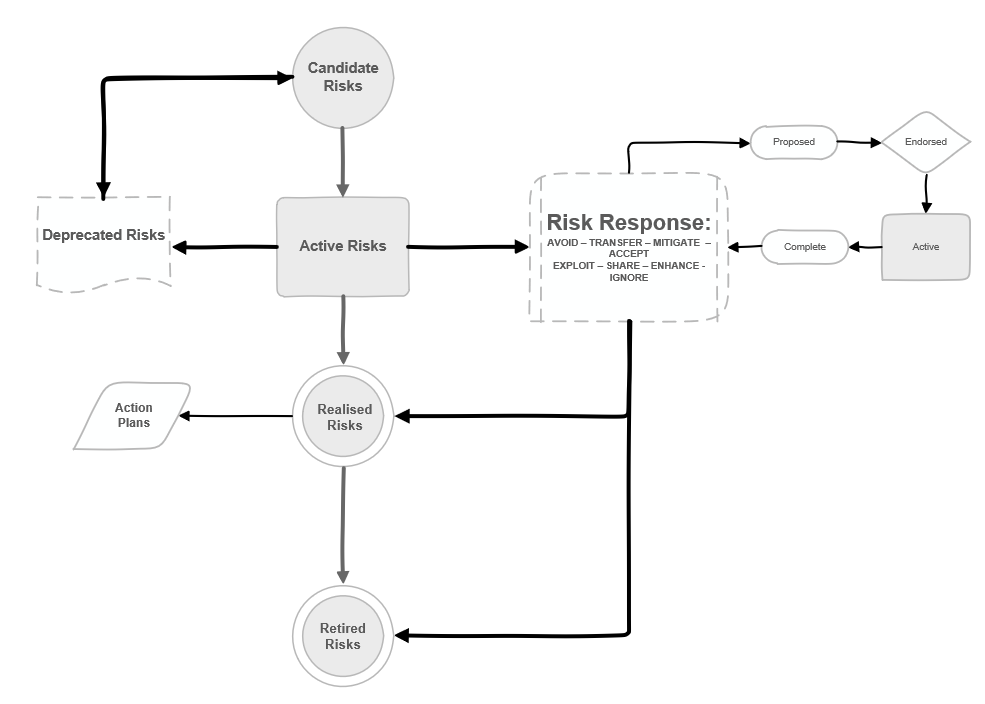
\includegraphics[width=\textwidth]{risk-lifecycle}
\label{fig:risk-lifecycle}
\end{figure}

\subsection{Terminology: Risk Categories}
\label{sec:risk-categories}

The following are categories and subcategories used to define risks in the Risk Register.

\begin{itemize}
	\item \textbf{Program Science} Category
		\begin{itemize}
			\item Astronomy and Astrophysics Community --- Priorities, needs and expectations of the community and the changes related to it.
			\item Science Related --- Science produced by the organization and its relevance and impact.
		\end{itemize}
	\item \textbf{Technical} Category
		\begin{itemize}
			\item Scope --- Related to Scope changes of the Organization/Project objectives.
			\item Requirements --- Identifying/missing/not well defined requirements.
			\item Processes --- Inadequate or not well defined technical or operational processes.
			\item Technology --- Technology readiness level and related.
			\item Interfaces --- Technical interfaces, infrastructure and complexity of the interfaces, and related.
			\item Quality --- Verification of the requirements and concept of operations, to ensure the performance. How well the as-built system compares against the requirements.
		\end{itemize}
	\item \textbf{Management} Category
		\begin{itemize}
			\item Program/Project Management --- Anything related to project and program like schedule, planning, monitoring and controlling.
			\item NOIRLab/AURA Management --- AURA, NOIRLab rates and other AURA and NOIRLab management related.
			\item Operations Management --- Portfolio Management, finance, ITOps, safety group, and other operations related.
			\item Resourcing --- Labor resourcing, shared resources availability, conflicts between fraction of shared resources.
			\item Communication --- Internal communication within the organization and external communication.
			\item Health \& Safety Environment --- Mental health of the employees due to pandemic, safety in the observatories, etc.
		\end{itemize}
	\item \textbf{Commercial/Organizational} Category
		\begin{itemize}
			\item Contractual/Procurement --- All contractual and procurement related events, liabilities, warranties, legal, compliance.
			\item Partnerships and Joint Ventures --- Any risks associated with tenants, partners and in-kind support, relationship.
			\item Subcontracts and Suppliers --- Any risk related to subcontractor and supplier issues (non-contractual); e.g., supplier going bankrupt.
		\end{itemize}
	\item \textbf{External} Category
		\begin{itemize}
			\item Financial --- All sources of risks related to funding and cash flow.
			\item Legislation and Regulatory --- Lease renewals, political, sites \& facilities, applicable law.
			\item Exchange Rates --- Exchange rates for currency, e.g., USD-CLP, USD-EUR.
			\item Natural Environmental Factors --- Risks related to weather, earthquakes, tsunami and other natural factors.
			\item Human Environmental Factors --- Risks related to light pollution, satellites, air pollution and other passive human factors.
			\item External Stakeholders --- External stakeholders influencing like funding agencies, public, protest group, hackers, hostile competitors or other active human factors.
		\end{itemize}
\end{itemize}

\subsection{Terminology: Risk Likelihood and Impact Categories}
\label{sec:risk-impact-tables}

This subsection includes the following tables to define risk likelihood categories and risk impact categories:
\begin{itemize}
	\item Table \ref{table:risk-likelihood} includes the definition of risk likelihood categories and corresponding percent chance.
	\item Table \ref{table:risk-overall-impacts} includes the definition of impact categories based on overall risk.
	\item Table \ref{table:risk-cost-impacts} includes the definition of impact categories based on cost.
	\item Table \ref{table:risk-schedule-impacts} includes the definition of impact categories based on schedule.
	\item Table \ref{table:risk-performance-impacts} includes the definition of impact categories based on performance.
\end{itemize}

\begin{table}[H]
\caption{Risk Likelihood Categories.}
\label{table:risk-likelihood}
\begin{tabular}{lll}
\multicolumn{1}{c}{\textbf{Likelihood Category}} & \multicolumn{1}{c}{\textbf{Percent Chance}} & \multicolumn{1}{c}{\textbf{Definition}} \\
Remote      & 10-20\% & Extremely unlikely to occur.                 \\
Unlikely    & 21-40\% & May occur only in exceptional circumstances. \\
Possible    & 41-60\% & Could occur in certain circumstances.        \\
Likely      & 61-80\% & Probably will occur in many circumstances.   \\
Very Likely & 81-90\% & Expected to occur in most circumstances.    
\end{tabular}
\end{table}

\begin{table}[H]
\caption{Risk Overall Impact Categories.}
\label{table:risk-overall-impacts}
\begin{tabular}{|c|l|}
\hline
\textbf{Impact Category} & \multicolumn{1}{c|}{\textbf{Overall Impact}}                                                                                                    \\ \hline
\textbf{Low}             & \begin{tabular}[c]{@{}l@{}}Any other impacts with respect to operations, project, or\\ initiative within the Programs or Services.\end{tabular} \\ \hline
\textbf{Moderate}        & \begin{tabular}[c]{@{}l@{}}Any impacts with respect to delivering an NOIRLab Program\\ or Service POP milestone.\end{tabular}                   \\ \hline
\textbf{Significant}     & \begin{tabular}[c]{@{}l@{}}Any impacts with respect to Key Performance Evaluation metric(s)\\ of an NOIRLab Program or Service.\end{tabular}    \\ \hline
\textbf{Damaging/Major}  & \begin{tabular}[c]{@{}l@{}}Any impacts with respect to priorities in the POP or LRP of\\ an NOIRLab Program or Service.\end{tabular}            \\ \hline
\textbf{Catastrophic/Extreme} &
  \begin{tabular}[c]{@{}l@{}}Any impacts with respect to NOIRLab Center CA and\\ Programs CSAs, and/or impacting the mission of NOIRLab or\\ any constituent Programs or Services.\end{tabular} \\ \hline
\end{tabular}
\end{table}

\begin{table}[H]
\caption{Risk Cost Impact Categories.}
\label{table:risk-cost-impacts}
\begin{tabular}{|c|l|}
\hline
\textbf{Impact Category}      & \multicolumn{1}{c|}{\textbf{Cost Impact}}                              \\ \hline
\textbf{Low}                  & Minimal consequence.                                                   \\ \hline
\textbf{Moderate}             & Cost variance less than or equal to 5\% of total approved FY baseline. \\ \hline
\textbf{Significant}    & \begin{tabular}[c]{@{}l@{}}Cost variance greater than 5\% but less than or equal to 10\% of total \\ approved FY baseline.\end{tabular} \\ \hline
\textbf{Damaging/Major} & \begin{tabular}[c]{@{}l@{}}Cost variance greater than 10\% but less than or equal to 15\% of total\\ approved FY baseline.\end{tabular} \\ \hline
\textbf{Catastrophic/Extreme} & Cost variance greater than 15\% of total approved FY baseline.         \\ \hline
\end{tabular}
\end{table}

\begin{table}[H]
\caption{Risk Schedule Impact Categories.}
\label{table:risk-schedule-impacts}
\begin{tabular}{|c|l|}
\hline
\textbf{Impact Category} & \multicolumn{1}{c|}{\textbf{Schedule Impact}} \\ \hline
\textbf{Low}             & Minimal consequence.                          \\ \hline
\textbf{Moderate} &
  \begin{tabular}[c]{@{}l@{}}Critical path does not slip; total slack of slipped tasks will not\\ impact critical path in less than 10 days.\end{tabular} \\ \hline
\textbf{Significant} &
  \begin{tabular}[c]{@{}l@{}}Critical path does not slip; total slack of slipped tasks is within\\ 10 days of impacting the critical path.\end{tabular} \\ \hline
\textbf{Damaging/Major}  & Critical path slips.                          \\ \hline
\textbf{Catastrophic/Extreme} &
  \begin{tabular}[c]{@{}l@{}}Critical path slips and one or more critical milestones or events\\ cannot be met.\end{tabular} \\ \hline
\end{tabular}
\end{table}

\begin{table}[H]
\caption{Risk Performance Impact Categories.}
\label{table:risk-performance-impacts}
\begin{tabular}{|c|l|}
\hline
\textbf{Impact Category} &
  \multicolumn{1}{c|}{\textbf{Performance Impact}} \\ \hline
\textbf{Low} &
  Minimal consequence to objectives/goals. \\ \hline
\textbf{Moderate} &
  Minor consequence to objectives/goals. \\ \hline
\textbf{Significant} &
  \begin{tabular}[c]{@{}l@{}}Unable to achieve a particular objective/goal, but remaining objective\\ goals represent better than minimum success or outcome.\end{tabular} \\ \hline
\textbf{Damaging/Major} &
  \begin{tabular}[c]{@{}l@{}}Unable to achieve multiple objectives/goals, but minimum success can\\ still be achieved or claimed.\end{tabular} \\ \hline
\textbf{Catastrophic/Extreme} &
  \begin{tabular}[c]{@{}l@{}}Unable to achieve objectives/goals such that minimum success cannot\\ be achieved or claimed.\end{tabular} \\ \hline
\end{tabular}
\end{table}


\section{Risk \& Opportunity Identification and Assessment}
\label{sec:id-assess}

This section describes who and how risks and opportunities are identified and assessed.
This is currently written assuming that the Risk Register is implemented in NOIRLab's ATS Risk Tool.

\begin{enumerate}
	\item The managing group creates a risk or opportunity in the Risk Register as a "Candidate."
	\item RROB reviews content, then either asks for more information or sets risk to "Active."
	\item After
\end{enumerate}

\subsection{Create Risk Item}

Minimum content before saving in the Risk Register:
\begin{itemize}
	\item Project --- Rubin Operations
	\item Risk Type --- Threat or Opportunity
	\item Risk Department --- Select Rubin Observatory department which owns the risk and its assessment
	\item Risk Owner --- Point-of-contact for ownership and technical information regarding risk. Responsible for orchestrating the response to the risk.
	\item Risk Category --- Select from list (need to add list to RDO-71)
	\item Risk Title --- Short, descriptive title
	\item Risk Statement --- Description of risk, which must include the IF-THEN statement at a minimum.
	\item Status --- Automatically set as ``Candidate''
\end{itemize}

Optional fields:
\begin{itemize}
	\item Risk Sub Category --- Select from list (need to add list to RDO-71)
	\item Parent --- Any applicable Parent risks
\end{itemize}

Risks can be created as ``children'' of ``parent'' risks.
This is appropriate for a risk that is anticipated as being realized in separate time-ordered phases, or as distinct parallel events that each have their own impact.
The cost and schedule impact of the parent is the combined cost and schedule impact of its children, see the next section for details.

\subsection{RROB Candidate Risk Review}

Should be reviewed by the Risk Owner before submitting.
RROB to review for sufficiency and accuracy of information, to confirm ability of Risk Owner to manage effectively as an Active risk.

Minimum content before submitting a Candidate Risk for review by the RROB:
\begin{itemize}
	\item Cost Impact --- According to risk table (need to add risk table to RDO-71).
	\item Likelihood --- According to risk table (need to add risk table to RDO-71)
	\item Schedule Impact --- According to risk table (need to add risk table to RDO-71)
	\item Cost and/or Schedule Impact Description
	% if over certain severity. PJM: I think we always want a brief description of any impact we specify.
	\item Cost and/or Schedule fields under Analyze Risk Quantitative, if impact is non-negligible.
	The Likely Cost is the estimated cost of addressing the risk in the year after it is realized.
	(All these short-term cost estimates are used to forecast the required annual level of reserve funds.)
	The Likely Delay is the estimated length of delay to the Impacted Milestone.
	If the Impacted Milestone is either ``Start of Operations'' or ``LSST Survey Completion,'' the Realized Risk Plan (see below) needs to include ``Extend Survey.''
	(Such schedule delays incur a post-ops cost.)
	\item Plan Type, and a minimum of one related Response Plan (i.e. how the risk will be mitigated)
	\item Realized Risk Plan --- Description of event trigger, and the plan for how the risk will be addressed once it is realized.
	\item All fields under Analyze Risk Quantitative --- note that these do not automatically populate any required fields.
	\item Existential Risk
\end{itemize}

Optional fields:
\begin{itemize}
	\item Overall Impact --- Impact category that can override the automatically generated cost and schedule impact categories (sets to most severe)
	% \item Cost or Schedule Impact Description. PJM: See above, I think we always need a description any time we specify an impact.
	\item Related Actions
\end{itemize}

Verify assessment in the automatically generated fields under Analyze Risk Score.

When analyzing a risk that is the parent of $N$ child risks:
\begin{itemize}
	\item First analyze the children separately, i.e. estimating Residual Probability $P_k$, Likely Cost $C_k$, and Likely Delay $S_k$ for the $k$-th risk, and repeating for all $k$ in the range $(1 \ldots N)$.
	\item For each risk, calculate the Cost Exposure $E_k = C_k \times P_k$.
	\item The combined Cost Exposure for the parent risk is just the sum of the Cost Exposures of its children, $E_{\rm total} = \sum_{k=1}^N E_k$.
	\item The Likely Cost of the parent risk is the sum of the Likely Costs of its children, $C_{\rm total} = \sum_{k=1}^N C_k$.
	\item The Residual Probability of the parent risk is its Cost Exposure divided by its Likely Cost, $P_{\rm total} = E_{\rm total} / C_{\rm total}$.
	This is just the cost-weighted average of the child risks' Residual Probabilities, and is the most meaningful definition of probability for parent risks.
	\item Other quantitative attributes of parent risks can be computed by simple summation (e.g. Minimum Cost, Maximum Delay, Schedule Exposure, etc).
	\item Pre-response quantities of parent risks, such as Impact Scores, can be reverse engineered from their Residual Probabilities.
\end{itemize}

\subsection{Continuous Review and Updates to Active Risks}

Risk Owners flag issues or proposed changes to Active Risks for review at an RROB monthly meeting.

Managing departments should review risks on a frequency based on severity.

In the (May) Annual Scrub, Level 3 Team Leaders are invited to review, in the Scrub Sandbox, pertinent fields of risks that their team is affected by and which they are expected to help respond to.
Modifications they propose are reviewed by the RROB and implemented in the Risk Register by the Risk Owners in the post-scrub implementation phase (June).

\subsection{Addressing Realized Risks}

Triggering a Realized Risk:
Review of all Response Plans and Actions by Risk Owner, and follow-up review with department management.
Risk Owner proposes change of Status from Active to Realized.
Review with RROB is required if severity is above threshold (determined by RROB Chair).

Addressing a Realized Risk:
Risk Owner works with department management to submit a Request Beyond Target (RBT) for additional resources needed to address the risk (see RTN-005 for the RBT process).
RBT is reviewed by RDO, which works with department for any needed escalation to NOIRLab, SLAC or the funding agencies or Resource Forum.

Additional resources for addressing risks are drawn from reserve funds.
The annual budget for the reserve is estimated as the sum of the cost exposure over all parent risks.
Currently, the cost exposure and budget calculations are performed outside the Risk Register in a companion tool (the ``Rubin View of the NOIRLab Risk Register'').

\subsection{Retiring Risks}

Review of close-out due to realized risk, or if event cannot trigger.
RROB to review before retiring risk that didn't trigger.
All actions should be completed in the Risk Register (could include Jira tickets for follow-up work) before retiring risk that did trigger.
Documentation updates should be considered.

\subsection{Risk Assessment}

There are six aspects to assessing the state of each risk and opportunity within a subsystem:
\begin{enumerate}
\item Identification:  identifying elements of risk in the department’s activity.
\item Establishing time frame:  determining the likely time at which an event would come to pass.
\item Assessing probability:  estimating the probability that an undesirable event may occur.
\item Assessing severity:  gauging the severity of the impact that such an event would have on the status of the project if the event were to occur.
\item Developing risk options:  developing plans to avoid, accept, mitigate, or transfer.
\item Developing a management response: consider how the project may respond if the event should occur.
\end{enumerate}


\section{Risk \& Opportunity Response\, Monitoring\, and Control}

This section describes how risks and opportunities responses, monitored and controlled.

\subsection {Risk \& Opportunity Response}

The definition of responses are included in the ATS Risk Software.
The following include the definition of response plans to risks, and additional comments are included in \href{RTN-051.lsst.io}.

\begin{itemize}
	\item \textbf{Avoid} ---
	changing your strategy or plans to avoid the risk. This risk response strategy is about removing the threat by any means. That can mean changing your management plan to avoid the risk because it’s detrimental to the project/program.

	\item \textbf{Transfer} ---
	passing ownership and/or liability to a third party - Transfer or pass the work on resolving the risk to a third party. For e.g. purchase fire insurance for an unfinished building.

	\item \textbf{Mitigate} ---
	reducing the probability and/or impact of the risk below a threshold of acceptability - Some risks cannot be avoided and need to take action to reduce the impact of the risk. For e.g. work procedures and equipment designed to reduce workplace safety risks.

	\item \textbf{Accept} ---
	recognizing residual risks and devising responses to control and monitor them - This risk response strategy consists of identifying a risk and documenting all the risk management information about it, but not taking any action unless the risk is realized. 
\end{itemize}

The following include the definition of response plans to opportunities.

\begin{itemize}
	\item \textbf{Exploit} ---
	Exploiting a risk to make use of the opportunity that becomes available if that risk occurs.

	\item \textbf{Share} ---
	Distributing the risk across multiple stakeholders (teams/projects/programs)

	\item \textbf{Enhance} ---
	Enhancements is an action that is taken to increase the chance of the opportunity occurring.

	\item \textbf{Ignore} ---
	Opportunities that cannot be actively addressed through exploiting, sharing or enhancing can perhaps be ignored, with no special measures being taken to address them.
\end{itemize}




\newpage

\appendix

% Include all the relevant bib files.
% https://lsst-texmf.lsst.io/lsstdoc.html#bibliographies
\section{References} \label{sec:bib}
\renewcommand{\refname}{} % Suppress default Bibliography section
\bibliography{local,lsst,lsst-dm,refs_ads,refs,books}

% Make sure lsst-texmf/bin/generateAcronyms.py is in your path
\section{Acronyms} \label{sec:acronyms}
\addtocounter{table}{-1}
\begin{longtable}{p{0.145\textwidth}p{0.8\textwidth}}\hline
\textbf{Acronym} & \textbf{Description}  \\\hline

DM & Data Management \\\hline
NOIRLab & NSF's National Optical-Infrared Astronomy Research Laboratory; \url{https://nationalastro.org} \\\hline
RDO & Rubin Directors Office \\\hline
SP & Story Point \\\hline
TBD & To Be Defined (Determined) \\\hline
\end{longtable}

% If you want glossary uncomment below and comment out the two lines above.
% \printglossaries

\end{document}
